
\chapter{Methods}




\section{Neuron and network model}

This section will go into detail about the computations behind the network which was developed by
\cite{sacramento2018dendritic} and expanded by \cite{Haider2021}.


\subsection{Network architecture}

\begin{figure}
  \centering
  \begin{minipage}{0.5\textwidth}
    \centering
    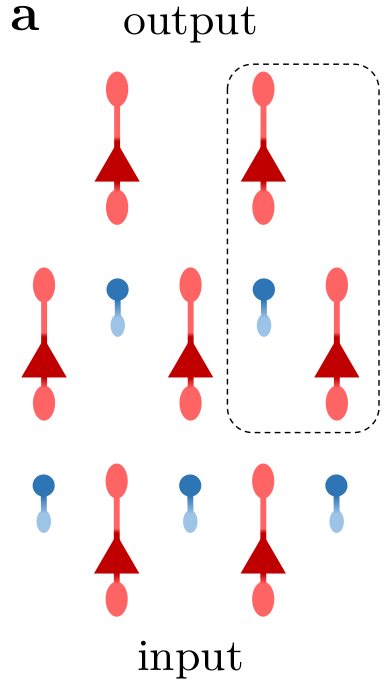
\includegraphics[width=0.9\textwidth]{network_a}
  \end{minipage}\hfill
  \begin{minipage}{0.4\textwidth}
    \centering
    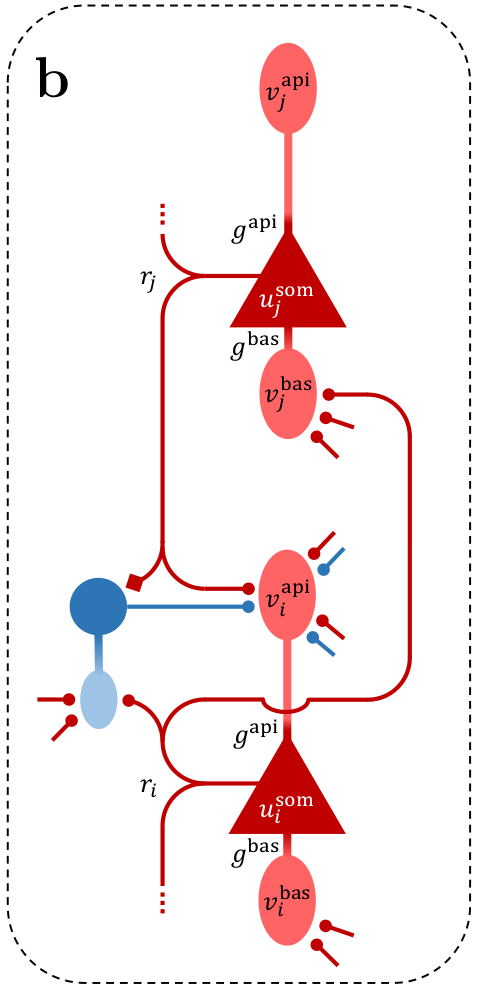
\includegraphics[width=0.9\textwidth]{network_b}
  \end{minipage}
  \caption{Network structure, from \cite{Haider2021}. \textbf{a:} pyramidal- (red) and interneurons (blue) in a network
    of three layers. Note the fact that the number interneurons in a layer is equal to the number of pyramidal neurons
    in the subsequent layer\protect\footnotemark. \textbf{b:} connectivity within the highlighted section. Feedback
    pyramidal-to-interneuron connections (displayed with rectangular synapse) transmit pyramidal somatic potential
    directly and connect to a single interneuron. This enables these interneurons to learn to match their corresponding
    next-layer pyramidal neurons. All other synapses (circles) transmit the neuron somatic activation $\phi (u^{som})$
    and fully connect their origin and target populations.}
  \label{fig-network}
\end{figure}

\footnotetext{{Note that the input layer is displayed as having interneurons here. This appears to be a mistake in the
      graphic. In the implementation, interneurons are only modelled in hidden layers.}}

The model which was original described by \cite{sacramento2018dendritic} contains a strongly recurrent network
structure, which will be explained in this section. It can be functionally separated into layers, with information
flowing from the input layer through one or more hidden layers to the output layer. Neurons at the input layer receive
no feedback connections and serve primarily to apply a low-pass filter over the input sequence injected into their
membrane. Output layers have no interneurons, and are usually modeled as pyramidal neurons without an apical
compartment. Hidden layers consist of a pyramidal- and an interneuron population, which are fully connected to each
other in both directions (see Figure \ref{fig-network}). Feedforward connections between layers are facilitated by
all-to-all connections between their respective pyramidal neurons and innervate the basal compartments. Feedback
connections from superficial layers and interneurons on the other hand arrive at apical compartments. Interneurons
receive lateral input from all pyramidal neurons of their layer, as well as feedback information from superficial
pyramidal neurons. These feedback connections are special, since they connect one pyramidal neuron to exactly one
interneuron. Instead of transmitting neuronal activation, this connection relays somatic voltage directly. The resulting
dynamics share features of electrical synapses, which will be discussed in Section \ref{sec-electric-syns}. To
understand what purpose this connectivity serves in our model, neuron and plasticity models require some elaboration.


\subsection{Neuron models}\label{sec-neurons}



The network contains two types of multi-compartment neurons; Pyramidal neurons with three compartments each, and
interneurons with two compartments each. They integrate synaptic inputs into dendritic potentials, which leak into the
soma with specific conductances. Note that vector notation will be used throughout this section, and $u_l^P$ and $u_l^I$
denote the column vectors of pyramidal- and interneuron somatic voltages respectively. Synaptic weights $W$ are likewise
assumed matrices.The activation $r_l^P$ of pyramidal neurons at layer $l$ is given by applying the synaptic transfer
function $\phi$ to to their somatic potentials $u_l^P$:
\begin{align}
  r_l^P   & = \phi(u_l^P)                                                        \\
  \phi(x) & = \begin{cases}
                0                                   & \textrm{if } \ x < -\epsilon \\
                \gamma \ log(1+e^{\beta(x-\theta)}) & \textrm{if } \ x < \epsilon  \\
                \gamma \ x                          & \textrm{otherwise}
              \end{cases}
\end{align}

where $\phi$ acts componentwise on $u$ and can be interpreted as a smoothed variant of ReLu \todo{cite} with scaling
factors $\gamma$, $\beta$, $\theta$ and threshold parameter $\epsilon$. The derivative somatic membrane potentials of
layer $l$ pyramidal neurons is given by:

\begin{align}
  C_m \dot{u}_l^P & = - g_l u_l^{som} + g^{bas} v_l^{bas} + g^{api} v_l^{api}
\end{align}

where $v_i^{bas}$ and $v_i^{api}$ are the membrane potentials of basal and apical dendrites respectively, and $g^{bas}$
and $g^{api}$ their corresponding coupling conductances. The membrane capacitance $C_m$ is $1$ in all relevant
simulations, and will be omitted from all Equations from here on out.


In the original model, dendritic compartments have no persistence between simulation steps. Thus, they are defined at
every timestep $t$ through incoming weight matrices and presynaptic activities:

\begin{align}
  v_l^{bas}(t) & = W_l^{up} \ \phi(u_{l-1}^P(t))                                     \\
  v_l^{api}(t) & =  W_l^{pi} \ \phi(u_l^I(t)) \ + \  W_l^{down} \ \phi(u_{l+1}^P(t))
\end{align}

Weight nomenclature conforms to the python implementation of the network by \cite{Haider2021}; Weights are indexed by
the layer in which the target neuron is located and belong to one of four populations. Feedforward and feedback
pyramidal-to-pyramidal connections arriving at layer $l$ are denoted $W_l^{up}$ and $W_l^{down}$ respectively. Lateral
pyramidal-to-interneuron connections are denoted with $W_l^{ip}$ and their corresponding feedback connections with
$W_l^{pi}$. Since the input layer contains no synapses, indexing begins with $0$ for the first hidden layer. \newline

Interneurons integrate synaptic information by largely the same principle, but instead of feedback information arriving
at the apical compartment, it is integrated directly into the soma. Through this, interneurons functionally resemble the
original neuron from \cite{urbanczik2014learning} most closely.

\begin{align}
  C_m \dot{u}_l^I & = - g_l u_l^{I} + g^{dend} v_l^{dend} + i^{nudge, I}\label{eq-intn-dynamics} \\
  i^{nudge, I}    & = g^{nudge, I} u_{l+1}^P                                                     \\
  v_l^{dend}      & = W_l^{ip} \ \phi(u_{l}^P)
\end{align}

where $ g^{nudge, I}$ is the interneuron nudging conductance, and $u_{l+1}^P$ is the somatic voltage of a corresponding
pyramidal neuron in the next layer. Since each interneuron is innervated by exactly one pyramidal neuron and vice versa,
they will be called each others \textbf{sister neurons} from here on.\todo{discuss whether this 1 to 1 style connection
  is plausible!}. Pyramidal neurons in the output layer $N$ effectively behave like interneurons, as they receive no input
to their apical compartment. Instead, the target  activation $u^{tgt}$ is injected into their soma:

\begin{align}
  C_m \dot{u}_N^P & = - g_l u_N^{P} + g^{bas} v_N^{bas} + i^{nudge, tgt} \\
  i^{nudge, tgt}  & = g^{nudge, tgt} u^{tgt}
\end{align}


These neuron dynamics correspond closely to those by \cite{urbanczik2014learning}, including the extension to more than
two compartments which was proposed in the paper. It should be noted however, that they are simplified in some key ways.
Primarily, dendritic couplings and nudging are not relative to the somatic or some reversal potential (i.e. $i^{nudge,
      tgt}= g^{nudge, tgt} (u^{tgt} - u_N^P )$), but are simplified to absolute values. \todo{Figure out if this makes a
  difference. maybe create a second branch to try them out? }








\section{Urbanczik-Senn Plasticity}\label{sec-urb-senn-plast}

The synapses in the network are all modulated according to variations of the "Urbanczik-Senn" plasticity rule
\citep{urbanczik2014learning}, which will be discussed in this section. \todo{add paragraph about relevance of
  urbanczik-senn}

The plasticity rule requires the postsynaptic neuron to have one somatic and at least one dendritic compartment, to the
latter of which synapses connect. The membrane potential of the dendritic compartment leaks into the somatic compartment
as described in Equation \ref{eq-intn-dynamics}.


Functionally, the plasticity rule changes the synaptic weight in such a way, as to minimize discrepancies between
somatic and dendritic potential. The change in weight for a synapse fron neuron $j$ to neuron $i$ is thus given by:

\begin{align}
  \dot{w}_{ij}    & = \eta \ ( \phi(u_i^{som}) - \phi(\hat{v}_i^{bas}) ) \ \phi(u_j^{som})^T \\
  \hat{v}_i^{bas} & = \alpha \  v_i^{bas}
\end{align}

with learning rate $\eta$ and $u^T$ denoting the transposition of the vector $u$ (which is by default assumed to be a
column vector). The dendritic prediction is simply a scaled version of the dendritic potential by the constant factor
$\alpha$, which is calculated from coupling and leakage conductances. For example, basal dendrites of pyramidal neurons
in \cite{sacramento2018dendritic} are attenuated by $\alpha = \frac{g^{bas}}{g_l + g^{bas} + g^{api}}$. If a current is
injected into the soma, it creates a difference between somatic firing rate and dendritic prediction (referred to as a
dendritic error from here on). \cite{urbanczik2014learning} show, that \todo{what?}





Weight changes for the synapses in a hidden layer $l$ are thus given by:

\begin{align}
  \dot{w}_{l}^{up}   & = \eta_l^{up} \ ( \phi(u_l^{P}) - \phi(\hat{v}_l^{bas}) ) \ \phi(u_{l-1}^{P})^T\label{eq-delta_w_up} \\
  \dot{w}_{l}^{ip}   & = \eta_l^{ip} \ ( \phi(u_l^{I}) - \phi(\hat{v}_l^{dend}) ) \ \phi(u_{l}^{P})^T\label{eq-delta_w_ip}  \\
  \dot{w}_{l}^{pi}   & = \eta_l^{pi} \ - v_l^{api} \ \phi(u_l^{I})^T\label{eq-delta_w_pi}                                   \\
  \dot{w}_{l}^{down} & = \eta_l^{down} \ ( \phi(u_l^{P}) - \phi(\hat{v}_l^{api}) )\ \phi(u_{l+1}^{P})^T
\end{align}

Note that pyramidal-to-pyramidal feedback weights $w_l^{down}$ are not plastic in most simulations, and are only listed
here for the sake of completeness \todo{some notes in the appendix to this?}




\section{The self-predicting network state}

In this model, euron dynamics, plasticity rules and network architecture form an elegant interplay, which I expand on in
this section. We will

Since each interneuron receives a somatic nudging signal from its corresponding next-layer pyramidal neuron, incoming
synapses from lateral pyramidal neurons adapt their weights to match feedforward pyramidal-to-pyramidal weights. In
intuitive terms; Feedforward pyramidal-to-pyramidal weights elicit a certain activation in the subsequent layer, which
is fed back into corresponding interneurons. In order to minimize the dendritic error term in Equation
\ref{eq-delta_w_ip}, pyramidal-to-interneuron weight matrices at every layer must match these forward weights ($w_l^{ip}
  \approx \omega w_l^{up}$) up to some scaling factor $\omega$. $\omega$ depends on the difference in parameters between
pyramidal- and interneurons, and is close to $1$ for most of the simulations considered here. As long as no feedback
information arrives at the pyramidal neurons, the Urbanczik-Senn plasticity drives synaptic weight to fulfill this
constraint. Note, that this alignment of two separate sets of outgoing weights is acheived with only local information.
Therefore this mechanism could plausibly align the weights of biological synapses that are physically separated by long
distances. \newline

Next, consider the special case for interneuron-to-pyramidal weights in Equation \ref{eq-delta_w_pi}, in which
plasticity does not serve to reduce discrepancies between dendritic and somatic potential. The error term is instead
defined solely by the apical compartment voltage\footnote{In strict terms, it is defined by the deviation of the
dendritic potential from its specific reversal potential. Since that potential is zero throughout, $- v_l^{api}$ remains
as the error term.}. Thus, plasticity in these synapses works towards silencing the apical compartment. The apical
compartments also receive feedback from superficial pyramidal neurons, whose synapses will be considered non-plastic for
now. As shown above, interneurons each learn to match their respective sister neuron activity. Thus, silencing of apical
compartments can only be acheived by mirroring the pyramidal-to-pyramidal feedback weights ($w_l^{pi} \approx
  -w_l^{down}$).\newline

When enabling plasticity in only these two synapse types, the network converges on the "\textbf{self-predicting state}"
\citep{sacramento2018dendritic}. This state is defined by a minimization of four error metrics at each hidden layer $l$:

\begin{itemize}
  \item The symmetries between feedforward ($w_l^{ip} \approx \omega w_l^{up}$) and feedback ($w_l^{pi} \approx
          -w_l^{down}$) weights. Mean squared error between these pairs of matrices will be called \textbf{Feedforward -
        } and \textbf{Feedback weight error} respectively.
  \item Silencing of pyramidal neuron apical compartments ($v_l^{api} \approx 0$). The Frobenius norm \citeme of apical
        compartment voltages within a layer is called the \textbf{Apical error}.
  \item Equal activations in interneurons and their respective sister neurons ($\phi (u_l^I) \approx \phi (u_{l+1}^P)$).
        The mean squared error over these vectors is called the \textbf{Interneuron error}.
\end{itemize}

\what{is there a mathematical symbol for this type of convergence?}

All of these equalities are approximate, since the network does not ever reach a state in which all of these values are
zero. In the original implementation, these deviations are minute and can likely be explained with floating point
conversions. Since it is impossible to replicate the timing of the original precisely within NEST, the NEST simulations
deviate more strongly from this ideal. The key insight here is, that this state is not clearly defined by absolute error
thresholds, but is rather flexible. Thus, networks are able to learn successfully even when their weights are
initialized imperfectly. \todo{or not at all? some science is required here}

An analysis of the equations describing the network reveals that the self-predicting state is stable \phrasing. When
Interneuron error is zero, dendritic and somatic compartments of all interneurons are equal, thus effectively disabling
plasticity in incoming synapses. Likewise, a silenced apical compartment will disable plasticity in all incoming
synapses. Synapses from lateral interneurons (Equation \ref{eq-delta_w_pi}) only depend on the apical compartment
itself, thus can not change in this state. Similarly, the apical compartment is also the driving factor for the
dendritic error of feedforward synapses (Equation \ref{eq-delta_w_up}), since it affects somatic activity when
active\footnote{This feature is actually rather important when contemplating biological neurons using the Urbanczik-Senn
  plasticity. In the original paper, currents were injected directly into the soma to change the error term. The the
  introduction of a second dendrite which performs that very task is much more useful, as originally described by the
  authors. Whether interneurons could be modeled by the same principles will be discussed in Section \todo{talk about
    interneuron dendritic trees}}. Thus, all plasticiy in the network is disabled, and remains in the self-predicting state
regardless of the kind of stimulus injected into the input layer. This fact highlights another important property of
networks in this state. Notice, how information flows backwards through the network; All feedback signals between layers
ultimately pass through the apical compartments of pyramidal neurons. Thus, successful silencing of all apical
compartments implies that no information can travel backwards between layers (with the exception of interneurons
receiving top down signals). As a result, the network behaves strictly like a fully connected feedforward network
consisting only of pyramidal neurons. The recurrence within this network is in balance, and completely cancels out its
own effects. This holds true as long as all conditions for the self-predicting state are fulfilled, and the network only
receives external stimulation at the input layer. One interpretation of this is, that the network has learned to predict
its own top-down input. A failure by interneurons to fully explain (i.e. cancel out) top-down input thus results in a
prediction error, encoded in deviation of apical dendrite potentials from their resting state. This prediction error in
turn elicits plasticity in all synapses connecting to its pyramidal neuron, which drives the network towards a
self-predicting state that is congruent with the novel top-down signal. Therefore, these neuron- specific prediction
errors are the driving force of supervised learning in these networks



\section{Training the network}

Starting with a network in the self-predicting state, performing time-continuous supervised learning then requires an
injection of a target activation into the network's output layer alongside with a stimulus at the input layer. Since
output layer neurons feed back into both interneurons and pyramidal neurons of the previous layer, local prediction
errors arise. Synapses activatee and drive to minimize the prediction errors, which requires the network to replicate
the target activation from activations and weights of the last hidden layer.

Note, that this mechanism is not exclusive to the last two layers. Any Apical errors cause a change in somatic activity,
which previous layers will fail to predict. Thus, errors are propagated backwards through the entire network, causing
error minimization at every layer. See the Supplementary analysis of \cite{sacramento2018dendritic} for a rigorous proof
that this type of network does indeed approximate the Backpropagation algorithm \what{what does the $\mathit{O}$ mean?}.



Classical backpropagation relies on a strict separation of a forward pass of some trainig pattern and a backwards pass
dependent on the loss produced at the output layer. Since this network is time-continuous, stimulus and target
activation are injected into the network simultaneously. These injections are maintained for a given presentation time
$t_{pres}$, in order to allow the network to calculate errors through its recurrent connections before slowly adapting
weights. Particluarly for deep networks, signals travelling from both the input and output layer require some time to
balance out and elicit the correct dendritic error terms. The network tends to overshoot activations, which in turn can
lead to poor learning performance with high learning rates. This issue will be discussed in more detail in Section
\ref{sec-haider}.



\section{NEST implementation}

One of the key research questions motivating this thesis is whether the proposed architecture would be able to learn
successfully when employing spike-based communication instead of the rate connections for which the original implementation
was developed. As a framework for my spike-based implementation two options were considered: The first one was to use the existing
implementation of the network within PyTorch \what{cite this or nah?} and expand it to employ spiking neurons. PyTorch
does in principle support spiking communication between layers, but is streamlined for implementing less recurrent
and less complex network and neuron models. A more pressing issue yet is efficiency. PyTorch is very well optimized for
efficiently computing matrix manipulations on dedicated hardware. Spiking communication is almost antithetical to this
design philosophy and thus can be expected to perform comparatively poor when using this backend.

The second option was to use the NEST simulator \citeme, which was developed with highly parallel simulations of large
SNN in mind. It is written in C++ and uses the \textit{Message Passing Interface} to efficiently communicate payloads
across both processes and compute nodes. 
Its key 

To calculate a number of spikes from the rate $r = \phi(u)$ , a poisson point process was used:

\begin{align}
  P\{\textit{n} \ \text{spikes during} \ \Delta t\} & = e^{-r \Delta t} \frac{(r \ \Delta t) ^ n}{n!}\label{eq-pr-n-spikes} \\
  \langle \textit{n} \rangle                        & = r \ \Delta t
\end{align}

with number of spikes \textit{n} and simulation timestep $\Delta t$, which will be assumed to be $0.1 ms$ from here on
out. Within the code, true number of spikes during $\Delta t$ is drawn from a poisson distribution with parameter
$\langle n \rangle$. Note that this mechanism makes the assumption that more than one spike can occur per simulation
step. NEST was developed with this possibility in mind, and handles such high rates without issue. Yet for the analysis
with regard to biological plausibility, spiking behaviour with refractory periods might be useful. The probability of at
least one spike occuring within the next simulation step thus is the inverse probability of no spike occuring. Entering
$n=0$ into Equation \ref{eq-pr-n-spikes}, the probability of eliciting at least one spike within the next simualtion
step becomes:

\begin{align}
  P\{ \textit{n} \geq 1\} & = 1 - e^{-r \Delta t}
\end{align}


After randomly drawing from this probability a spike is sent, and the spiking probability is set to 0 for the duration
of the refractory period $t_{ref}$.

\section{Event-based Urbanczik-Senn plasticity}\label{sec-event-urb}

One major challenge in implementing this architecture with spiking neurons is the Urbanczik-Senn plasticity as introduced
in Section \ref{sec-urb-senn-plast}. This problem has been successfully solved in NEST by \cite{Stapmanns2021} for the
two-compartment neurons described in \cite{urbanczik2014learning}. This Section will discuss its algorithm and
implementation.

Since it
depends on pre- and postsynaptic information for all updates, one of two approaches is typically employed to compute it:

One option is to store all relevant state variables for every timestep in the synapse and update the synaptic weight
whenever a spike is sent through the synapse. This is efficient in terms of computation time, since fewer computations are
required per synapse. The major downside of the approach lies in memory efficiency; Every synapse potentially stores the
history over several hundred simulation steps. In addition, every synapse innervating a given neuron would store its
membrane potentials redundantly.

Another approach updates synaptic weights at every timestep. This requires very little memory, but substantially
increases computation time. Importantly, it is poorly suited for asynchronous neuron simulations, as all synapses and
their weights need to be updated at every simulation step sequentially for their target neuron. In particular for large
networks and modern hardware
solutions, asynchronous simulations have proven to be more efficient for many use cases \todo{cite something by abigail}

Thus, a novel approach was developed by \cite{Stapmanns2021} for the NEST simulator, which will be explained in this
section. In order to utilize the paralellization capabilities of NEST and spiking neural networks, transmitting the pre-
and postsynaptic membrane potential is a poor choice. Thus, the error between somatic and dendritic activation is stored
in the \texttt{urbanczik\_history} of the postsynaptic neuron. Since it applies equally to all incoming synapses,
redundant storage is avoided by storing an access counter alongside each entry. Whenever an incoming syna



\begin{align}
  \kappa(t) & = H(t)e^{-t/\tau_{\kappa}} \\
  H(t)      & =
  \begin{cases}
    1 & \text{if $t > 0$}    \\
    0 & \text{if $t \leq 0$} \\
  \end{cases}
\end{align}

Antiderivatives:

\begin{align}
  \int_{-\infty}^x H(t)dt = tH(t) = max(0,t)
\end{align}

Convolution:

\begin{align}
  (f \ast g)(t) & = \int_{- \infty }^{\infty} f(\tau) g(t-\tau) d \tau
\end{align}
For functions f, g supported on only $[0, \infty]$ (as one-sided decay kernels and spiketrains are), integration limits
can be truncated:
\begin{align}
  (f \ast g)(t) & = \int_{0}^{t} f(\tau) g(t-\tau) d \tau \\
\end{align}


Plasticity:

\begin{align}
  \frac{dW_{ij}}{dt}(t) & = F(W_{ij}(t), s_i^\ast (t), s_j^\ast (t), V_i^\ast (t)) \\
  F[s_j^\ast, V_i^\ast] & = \eta \kappa \ast (V_i^\ast s_j^\ast)                   \\
  \text{with } V_i^\ast & = (s_i - \phi(V_i )) h(V_i),                             \\
  s_j^\ast              & = \kappa_s \ast s_j.
\end{align}

For an event-based plasticity we need:

\begin{align}
  \Delta W_{ij}(t,T) & = \int_t^T dt' F[s_j^\ast , V_i^\ast ](t')                                                 \\
                     & = \int_t^T dt' \eta \kappa \ast (V_i^\ast s_j^\ast)                                        \\
                     & = \eta \int_t^T dt' \  \int_0^{t'} dt'' \ \kappa(t'-t'') V_i^\ast (t'') s_j^\ast (t'')     \\
                     & = \eta \int_0^t dt' \  \int_{t''}^{t'} dt'' \ \kappa(t'-t'') V_i^\ast (t'') s_j^\ast (t'') \\
\end{align}


Starting with the complete Integral from $t=0$.

\begin{align}
  \Delta W_{ij}(0,t) & =\eta \int_0^t dt' \  \int_0^{t'} dt'' \ \kappa(t'-t'') V_i^\ast (t'') s_j^\ast (t'')                          \\
                     & = \eta \int_0^t dt'' \  \int_{t''}^{t} dt' \ \kappa(t'-t'') V_i^\ast (t'') s_j^\ast (t'')                      \\
                     & = \eta \int_0^t dt'' \  \left[ \tilde{\kappa}(t-t'') - \tilde{\kappa}(0) \right] V_i^\ast (t'') s_j^\ast (t'') \\
\end{align}

With $\tilde{\kappa}$ being the antiderivative of $\kappa$:

\begin{align}
  \kappa(t)         & = \frac{\delta}{\delta t} \tilde{\kappa}(t) \\
  \tilde{\kappa}(t) & = - e^{-\frac{t}{t_{\kappa}}}               \\
\end{align}

The above can be split up into two separate integrals:
\begin{align}
  \Delta W_{ij}(0,t) & =\eta \left[ -I_2 (0, t) + I_1(0,t) \right]                                      \\
  I_1(t_1, t_2)      & = - \int_{t_1}^{t_2} dt' \ \tilde{\kappa} (0) V_i^\ast (t') s_j^\ast (t')        \\
  I_2(t_1, t_2)      & = - \int_{t_1}^{t_2} dt' \ \tilde{\kappa} (t_2 - t') V_i^\ast (t') s_j^\ast (t') \\
\end{align}

Which implies the identities

\begin{align}
  I_1(t_1, t_2 + \Delta t) & = I_1 (t_1, t_2) + I_1 (t_2, t_2 + \Delta t)                                       \\
  I_2(t_1, t_2 + \Delta t) & = e^{- \frac{t_2 - t_1}{\tau_{\kappa}}} I_2 (t_1, t_2) + I_2 (t_2, t_2 + \Delta t)
\end{align}


\begin{align}
  I_2 (t_1, t_2 + \Delta t) & = -\int_{t_1}^{t_2 + \Delta t} dt' \ \tilde{\kappa} (t_2 + \Delta t - t') V_i^\ast (t') s_j^\ast (t')                                        \\
                            & = -\int_{t_1}^{t_2} dt' \ \left[ -e^{- \frac{t_2 + \Delta t - t'}{\tau_\kappa}} \right] V_i^\ast (t') s_j^\ast (t')
  -\int_{t_2}^{t_2 + \Delta t} dt' \ \left[ -e^{- \frac{t_2 + \Delta t - t'}{\tau_\kappa}} \right] V_i^\ast (t') s_j^\ast (t')                                             \\
                            & = -e^{- \frac{ \Delta t}{\tau_\kappa}} \int_{t_1}^{t_2} dt' \ \left[ -e^{- \frac{t_2 - t'}{\tau_\kappa}} \right] V_i^\ast (t') s_j^\ast (t')
  -\int_{t_2}^{t_2 + \Delta t} dt' \ \left[ -e^{- \frac{t_2 + \Delta t - t'}{\tau_\kappa}} \right] V_i^\ast (t') s_j^\ast (t')
\end{align}


Using this we can rewrite the weight change from $t$ to $T$ as:


\begin{align}
  \Delta W_{ij}(t,T) & = \Delta W_{ij}(0,T) - \Delta W_{ij}(0,t)                                               \\
                     & = \eta [-I_2(0,T) + I_1(0,T) + I_2(0,t) - I_1(0,t)]                                     \\
                     & = \eta [I_1(t,T) - I_2(t,T) + I_2(0,t)\left( 1 - e^{- \frac{T-t}{\tau_\kappa}} \right)]
\end{align}

The simplified \cite{sacramento2018dendritic} case would be:

\begin{align}
  \frac{dW_{ij}}{dt} & = \eta (\phi(u_i) - \phi(\hat{v_i})) \phi(u_j)                                         \\
  \Delta W_{ij}(t,T) & = \int_t^T dt' \ \eta \  (\phi(u_i^{t'}) - \phi(\widehat{v_i^{t'}})) \  \phi(u_j^{t'}) \\
  \Delta W_{ij}(t,T) & = \eta \int_t^T dt' \  (\phi(u_i^{t'}) - \phi(\widehat{v_i^{t'}})) \ \phi(u_j^{t'})    \\
  V_i^*              & = \phi(u_i^{t'}) - \phi(\widehat{v_i^{t'}})                                            \\
  s_j^*              & = \kappa_s * s_j
\end{align}


Where $s_i$ is the postsynaptic spiketrain and $V_i^*$ is the error between dendritic prediction and somatic rate and
$h( u )$. The additional nonlinearity $h( u ) = \frac{d}{du} ln \  \phi(u)$ is ommited in our model \todo{should it
  though?}.



\begin{align}
  \tau_l & = \frac{C_m}{g_L} = 10 \\
  \tau_s & = 3
\end{align}

Writing membrane potential to history (happens at every update step of the postsynaptic neuron):

\begin{lstlisting}[language=C++, directivestyle={\color{black}}
                   emph={int,char,double,float,unsigned,exp},
                   emphstyle={\color{blue}}]

UrbanczikArchivingNode< urbanczik_parameters >::write_urbanczik_history(Time t, double V_W, int n_spikes, int comp)
{
	double V_W_star = ( ( E_L * g_L + V_W * g_D ) / ( g_D + g_L ) );
	double dPI = ( n_spikes - phi( V_W_star ) * Time::get_resolution().get_ms() )
      * h( V_W_star );
}\end{lstlisting}

I interpret this as:


\begin{align}
  \int_{t_{ls}}^T dt' \ V_i^* & = \int_{t_{ls}}^T dt' \  (s_i - \phi(V_i )) h(V_i),               \\
  \int_{t_{ls}}^T dt' \ V_i^* & = \sum_{t=t_{ls}}^T \  (s_i(t) -  \phi(V_i^t ) \Delta t) h(V_i^t) \\
\end{align}

\begin{lstlisting}[language=C++, directivestyle={\color{black}}
                   emph={int,char,double,float,unsigned,exp},
                   emphstyle={\color{blue}}]
for (t = t_ls; t< T; t = t + delta_t)
{
   	minus_delta_t = t_ls - t;
    minus_t_down = t - T;
    PI = ( kappa_l * exp( minus_delta_t / tau_L ) - kappa_s * exp( minus_delta_t / tau_s ) ) * V_star(t);
    PI_integral_ += PI;
    dPI_exp_integral += exp( minus_t_down / tau_Delta_ ) * PI;
}  
// I_2 (t,T) = I_2(0,t) * exp(-(T-t)/tau) + I_2(t,T)
PI_exp_integral_ = (exp((t_ls-T)/tau_Delta_) * PI_exp_integral_ + dPI_exp_integral);
W_ji = PI_integral_ - PI_exp_integral_;
W_ji = init_weight_ + W_ji * 15.0 * C_m * tau_s * eta_ / ( g_L * ( tau_L - tau_s ) );    
  
kappa_l = kappa_l * exp((t_ls - T)/tau_L) + 1.0;
kappa_s = kappa_s * exp((t_ls - T)/tau_s) + 1.0;
  \end{lstlisting}


\begin{align}
  \int_{t_{ls}}^T dt' s_j^* & =  \tilde{\kappa_L}(t') * s_j -  \tilde{\kappa_s}(t') * s_j
\end{align}

$I_1$ in the code is computed as a sum:

\begin{align}
  I_1 (t,T) = \sum_{t'=t}^T \ (s_L^*(t') - s_s^*(t')) * V^*(t')
\end{align}


\section{Neuron model adaptations}

\begin{itemize}
  \item additional compartments
  \item top-down plasticity changes
  \item leaky dendrites
  \item pyr and intn differences
  \item
\end{itemize}

\begin{align}
  u_k^p           & = \frac{g_B}{g_{lk} + g_B + g_A} v^P_{B,k} + \frac{g_A}{g_{lk} + g_B + g_A} v^P_{A,k} \\
  \hat{v}^P_{B,k} & = \frac{g_B}{g_{lk} + g_B + g_A} v^P_{B,k}                                            \\
  \hat{v}^I_{k}   & = \frac{g_B}{g_{lk} + g_B} v^I_{k}                                                    \\
  \lambda         & = \frac{g_{som}}{g_{lk} + g_B + g_{som}}
\end{align}



\section{Haider 2021 updates}\label{sec-haider}

Besides the using a prediction of future somatic activity for neuronal transfer and plasticity, \cite{Haider2021} also
slightly alter the plasticity rule, which turns out to be crucial for the latent equilibrium mechanism. While the
simulations by \cite{sacramento2018dendritic} use the equations above, the new implementation
\href{https://github.com/neurips}{fill with neurips link} implicitly change them within its code. The fundamental
building block of a network here is a layer, which is represented in code as an instance of the class \texttt{Layer}.
Each instances holds information about its corresponding pyramidal- and interneurons. It also holds information about
the synaptic connections between the two populations, as well as all incoming feedforward and feedback pyramidal
synapses. A layer has two class methods that are fundamental to its computation; \texttt{update()} computes membrane
potential derivatives and synaptic weight changes given pyramidal neuron activations from the previous and subsequent
layers. \texttt{apply()} updates weights and membrane potentials from the previously calculated changes. Layers are
processed in order from input to output layer, where all of them receive the \texttt{update()} signal first, before
\texttt{apply()} is called on all of them. This ordering ensures, that changes in activation do not cascade through the
layers and lead to excessive activations at the output. Yet, since next layer activations at time $t$ have not been
computed, top down information is always delayed by one timestep.
\todo{evaluate importance of this}


Thus, the equations for membrane updates change slightly:

\begin{align}
  \dot{W_{ij}}(t)    & = \eta (\phi(u_i) - \phi(\alpha v^{basal}_i(t))) \phi(u_j)                             \\
  \Delta W_{ij}(t,T) & = \int_t^T dt' \ \eta \  (\phi(u_i^{t'}) - \phi(\widehat{v_i^{t'}})) \  \phi(u_j^{t'}) \\
  \Delta W_{ij}(t,T) & = \eta \int_t^T dt' \  (\phi(u_i^{t'}) - \phi(\widehat{v_i^{t'}})) \ \phi(u_j^{t'})    \\
  V_i^*              & = \phi(u_i^{t'}) - \phi(\widehat{v_i^{t'}})                                            \\
  s_j^*              & = \kappa_s * s_j
\end{align}



\section{Latent equilibrium}

\begin{align}
  \phi(V^{som}) & \rightarrow \phi(\breve{V}^{som}) \\
  \breve{V}     & := V + \tau^m \dot{V}             \\
\end{align}
\begin{align}
  \frac{d}{dt} W_{ba} & = \eta (\phi(V_b^{som}) - \phi(\alpha V_b^{dend})) \phi(V_a^{som})                         \\
  \frac{d}{dt} W_{ba} & = \eta (\phi(\breve{V}_b^{som}) - \phi(\alpha \breve{V}_b^{dend})) \phi(\breve{V}_a^{som})
\end{align}


\section{rate neurons in NEST}

\section{simulation details/updates}

All voltages need to be reset between simulations!

\begin{itemize}
  \item injections into the network
  \item output layer readout
  \item interoperability of networks
  \item 

\end{itemize}

